
%(BEGIN_QUESTION)
% Copyright 2006, Tony R. Kuphaldt, released under the Creative Commons Attribution License (v 1.0)
% This means you may do almost anything with this work of mine, so long as you give me proper credit

Suppose you see this label on a chemical storage container:

$$\includegraphics[width=15.5cm]{i00585x01.eps}$$

This is a standardized label (National Fire Protection Association -- NFPA) identifying certain hazards of the chemical stored in the container.  Identify what all the markings on this label mean.

\underbar{file i00585}
%(END_QUESTION)





%(BEGIN_ANSWER)

This chemical is rated ``extremely hazardous,'' with a flash point somewhere between 100$^{o}$ F and 200$^{o}$ F, and may detonate under normal conditions.  Additionally, it is dangerous if it contacts water.

\vskip 10pt

The left-hand (blue) diamond rates the substance according to its human health hazard:

\begin{itemize}
\item{} 0 = No hazard
\item{} 1 = Slight hazard
\item{} 2 = Moderately hazardous
\item{} 3 = Extremely hazardous
\item{} 4 = Deadly
\end{itemize} 

\vskip 10pt

The upper (red) diamond rates the substance according to its flammability (flash point):

\begin{itemize}
\item{} 0 = Will not burn
\item{} 1 = Above 200$^{o}$ F
\item{} 2 = Between 100$^{o}$ F and 200$^{o}$ F
\item{} 3 = Between 73$^{o}$ F (room temperature) and 100$^{o}$ F
\item{} 4 = Below 73$^{o}$ F (room temperature)
\end{itemize} 

\vskip 10pt

The right-hand (yellow) diamond rates the substance according to its chemical reactivity:

\begin{itemize}
\item{} 0 = Stable
\item{} 1 = Unstable if heated
\item{} 2 = Violent chemical change, no detonation
\item{} 3 = Shock or heat may detonate
\item{} 4 = May detonate under normal conditions
\end{itemize} 

\vskip 10pt

The lower (white) diamond is a place for abbreviations regarding additional properties.  Standardized abbreviations include:

\begin{itemize}
\item{} ACID = Acidic
\item{} ALK = Alkaline
\item{} COR = Corrosive
\item{} OX = Oxidizer
\item{} P = Polymerization (chemically reacts with itself under certain conditions)
\item{} W (with a line going through it) = Reacts with water
\end{itemize} 


%(END_ANSWER)





%(BEGIN_NOTES)

%INDEX% Chemistry, safety: NFPA hazard labels

%(END_NOTES)


